\documentclass{article}

\usepackage[utf8]{inputenc}
\usepackage{amsmath, esint}
\usepackage{amsfonts}
\usepackage[printonlyused]{acronym}
\usepackage{wasysym}
\usepackage[colorlinks]{hyperref}
\usepackage{lmodern}
\usepackage{graphicx}
\usepackage{xcolor}
\usepackage[left=2cm, top=3cm, right=2cm]{geometry}
\usepackage{booktabs}
\usepackage{tabularx}

\hypersetup{
  urlcolor=blue,
  linkcolor=black,
}

\title{\textbf{Final Project ML101} \\ From Pixels to Predictions: A Comparative Framework for Sentinel-2 Land-Cover Classification}
\author{Andrés Oswaldo Calderón Romero, Ph.D.}
\date{\today}

\begin{document}

\maketitle

\section{Introduction}
Modern geoinformatics has evolved from static cartography into a dynamic discipline essential for real-time environmental monitoring. This project offers a comprehensive framework for applying machine learning fundamentals to real-world scenarios, utilizing multispectral satellite imagery to quantify and analyze land cover. By integrating open-source tools with advanced machine learning architectures, this workflow moves beyond passive observation into rigorous spatial analysis. Mirroring professional GeoAI pipelines, model development and deployment are executed within specialized computational environments rather than traditional GIS software. Ultimately, this approach equips participants to bridge the gap between raw geospatial data and actionable environmental intelligence.

\section{Region of Interest (ROI)}
This project utilizes a multispectral scene from the Sentinel-2 satellite constellation, captured over Bogotá on August 10, 2026. Sentinel imagery is operated by the European Space Agency (ESA) under the Copernicus Earth observation program\footnote{\url{https://www.esa.int/Applications/Observing_the_Earth/Copernicus/Sentinel-2}}. Specifically, the dataset corresponds to a Level-2A product (Tile: T18NWL), which provides bottom-of-atmosphere reflectance.

The selected scene comprises 10 spectral bands spanning the visible, near-infrared (NIR), and short-wave infrared (SWIR) regions of the electromagnetic spectrum. While the native spatial resolutions of these bands vary (10m, 20m, and 60m), all image arrays in this specific dataset have been resampled to a uniform 20-meter spatial resolution to facilitate consistent pixel-level machine learning analysis. Figure~\ref{fig:roi} depicts the geographic extent of the study area.

\begin{figure}[htbp]
    \centering
    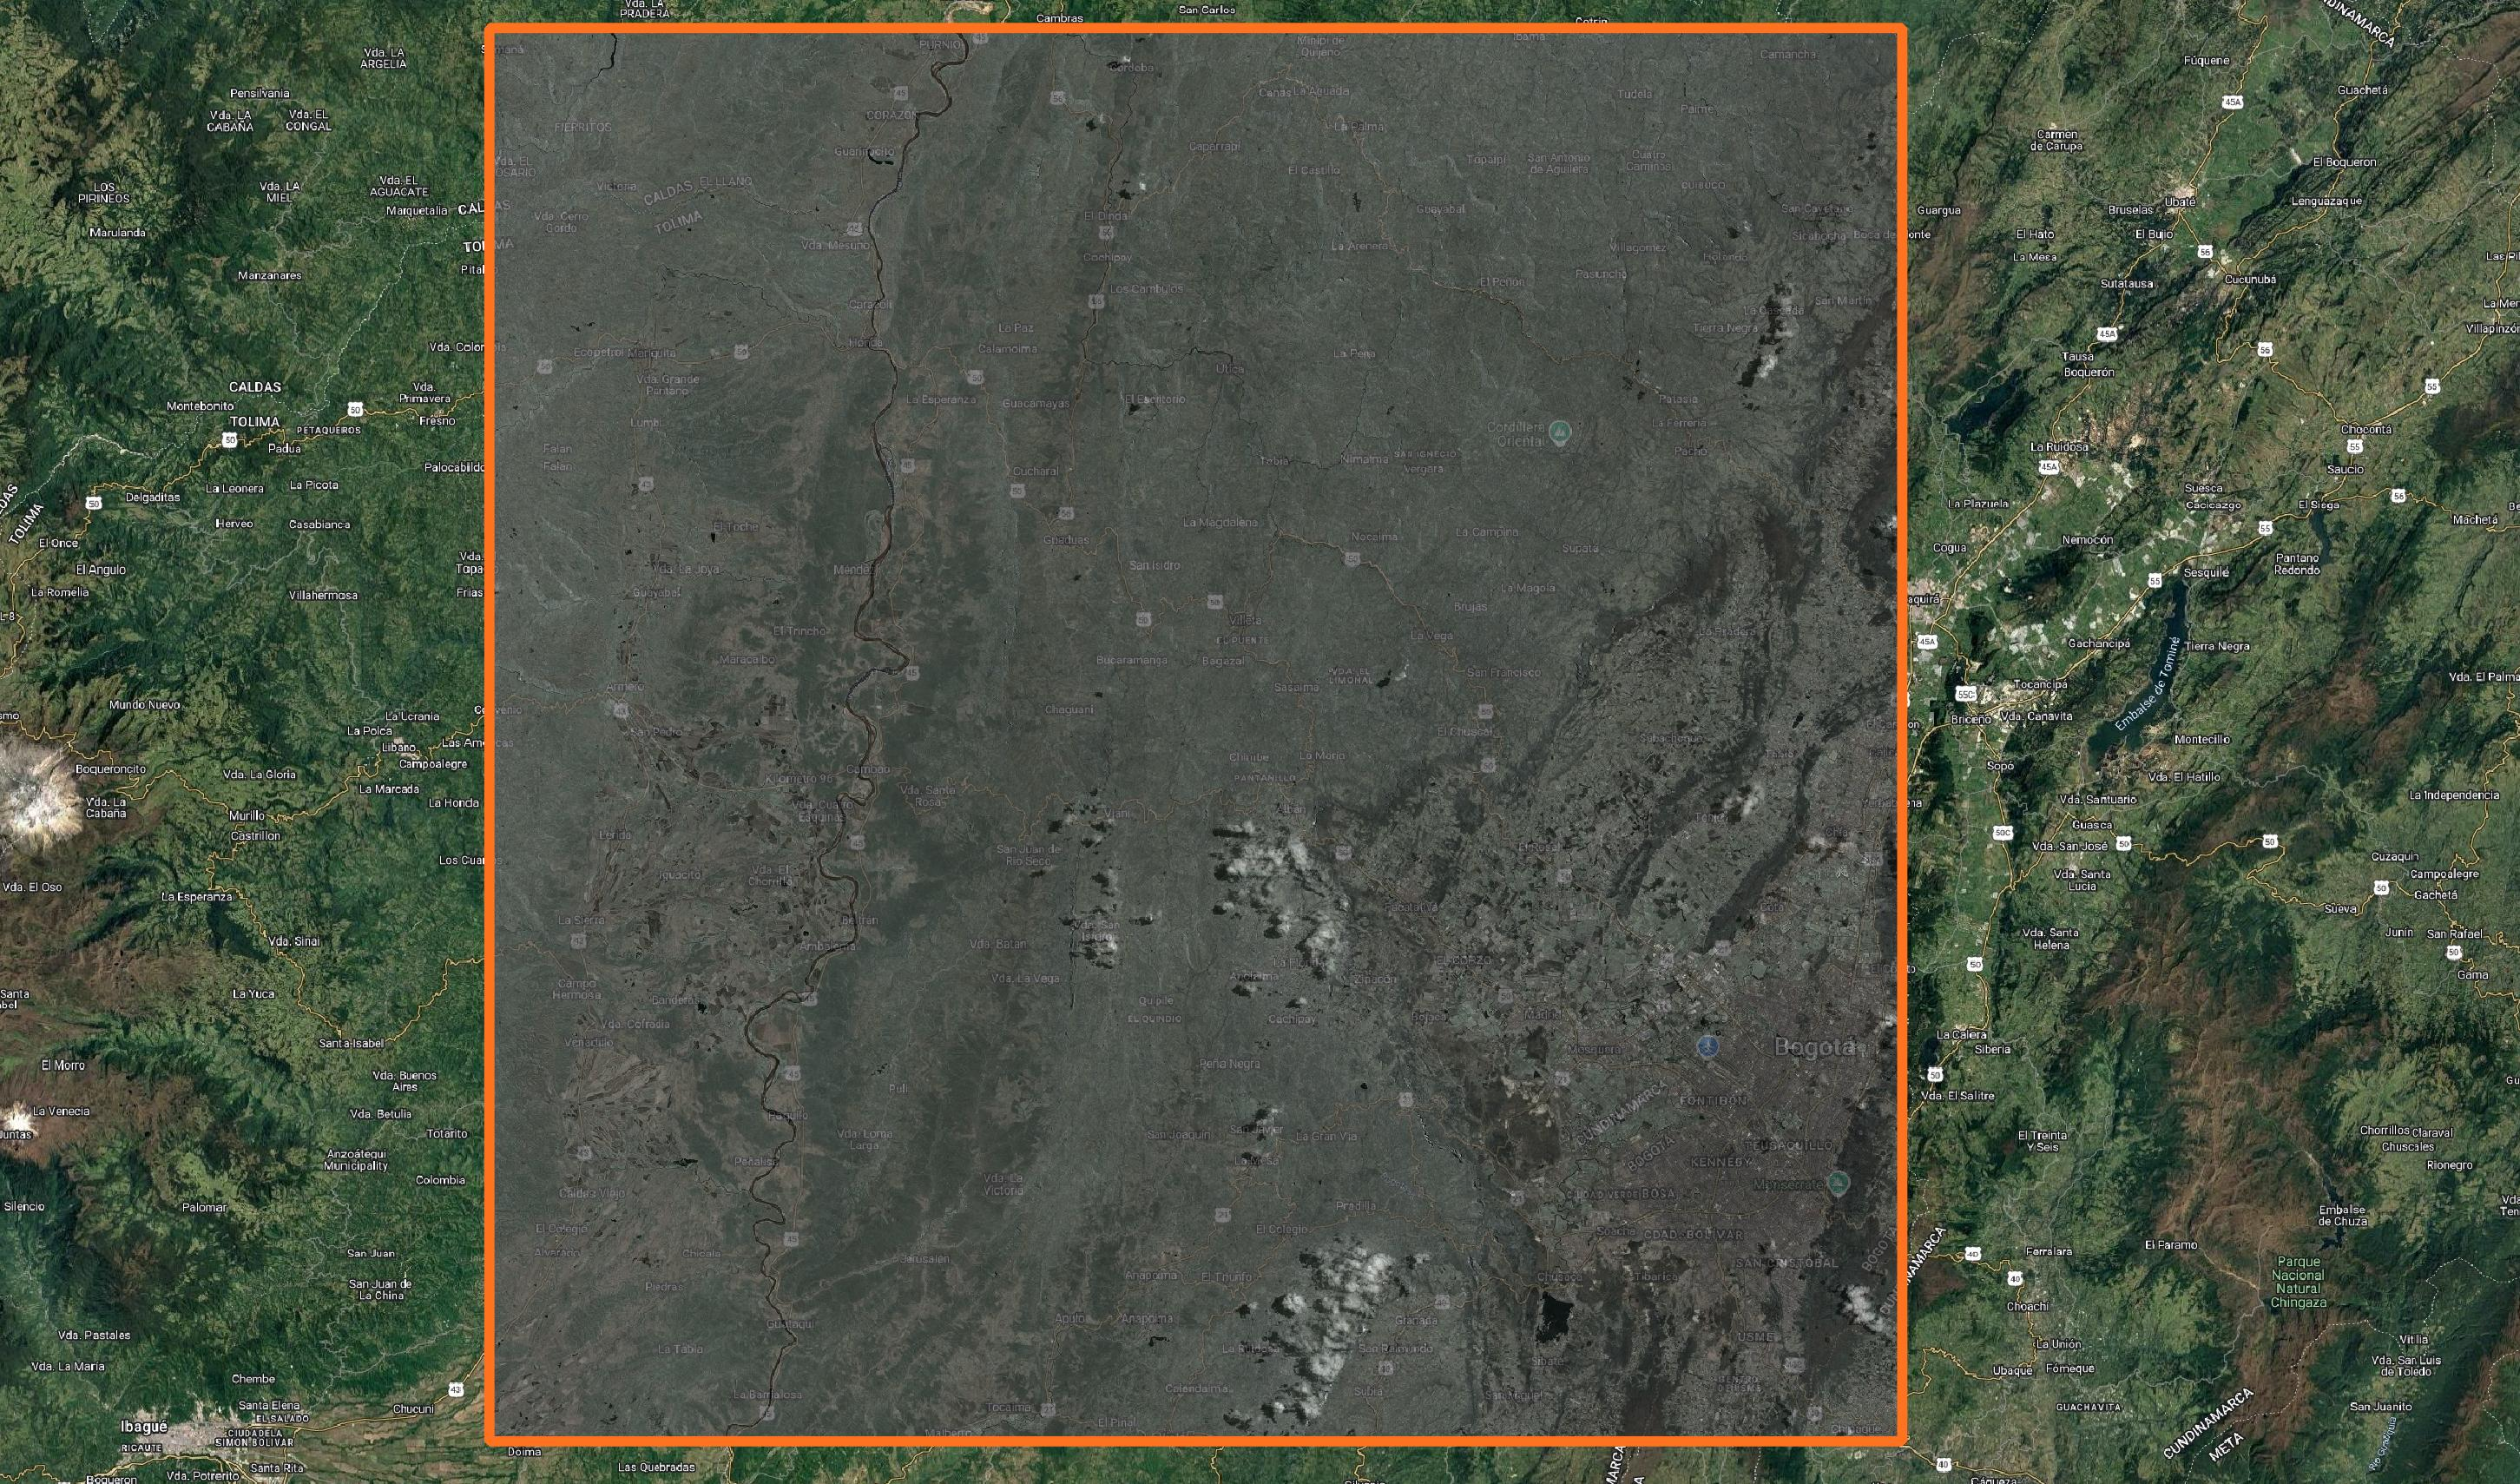
\includegraphics[width=\textwidth]{figures/roi}
    \caption{Geographic extent of the Sentinel-2 study area over Bogotá, Colombia.}
    \label{fig:roi}
\end{figure}

\subsection{Sentinel-2 Band Characteristics}

The dataset is expected to be derived from a Sentinel-2 Level-2A product\footnote{\url{https://custom-scripts.sentinel-hub.com/custom-scripts/sentinel-2/bands/}} (Tile: T18NWL, Date: August 10, 2026). Teams have access to the scene's imagery through the following \href{https://drive.google.com/drive/folders/1PcY6xgIXweaTyFkotvhcjVsLUVlv5oAY?usp=sharing}{link}.  The \texttt{\_20m.jp2} suffix appended to the filenames indicates that all included image arrays have been harmonized to a 20-meter spatial resolution. While certain bands natively possess 10-meter or 60-meter resolutions, this resampling process is a necessary preprocessing step to ensure dimensional consistency across the multi-dimensional feature space required for machine learning model training and inference.

Table~\ref{tab:bands} summarizes the physical properties of the selected spectral bands. This specific subset of 10 bands was chosen for its high utility in land-cover classification; for instance, the visible spectrum (B02--B04) captures basic color properties, the Red Edge bands (B05--B07, B8A) are critical for distinguishing vegetation health and types, and the Short Wave Infrared bands (B11, B12) provide essential data on moisture content and built-up surfaces.

\begin{table}[htbp]
    \centering
    \caption{Characteristics of the selected Sentinel-2 spectral bands. The dataset standardizes all inputs to a 20\,m file resolution to maintain a consistent matrix for pixel-level classification.}
    \vspace{0.5em}
    \renewcommand{\arraystretch}{1.3}
    \begin{tabularx}{\textwidth}{l X c c c}
        \toprule
        \textbf{Band} & \textbf{Description} & \textbf{Central Wavelength} & \textbf{Native Res.} & \textbf{File Res.} \\
        \midrule
        \textbf{B01} & Coastal aerosol              & 443 nm  & 60 m & 20 m \\
        \textbf{B02} & Blue                         & 490 nm  & 10 m & 20 m \\
        \textbf{B03} & Green                        & 560 nm  & 10 m & 20 m \\
        \textbf{B04} & Red                          & 665 nm  & 10 m & 20 m \\
        \textbf{B05} & Vegetation Red Edge          & 705 nm  & 20 m & 20 m \\
        \textbf{B06} & Vegetation Red Edge          & 740 nm  & 20 m & 20 m \\
        \textbf{B07} & Vegetation Red Edge          & 783 nm  & 20 m & 20 m \\
        \textbf{B8A} & Narrow NIR                   & 865 nm  & 20 m & 20 m \\
        \textbf{B11} & SWIR (Short Wave Infrared)   & 1610 nm & 20 m & 20 m \\
        \textbf{B12} & SWIR (Short Wave Infrared)   & 2190 nm & 20 m & 20 m \\
        \bottomrule
    \end{tabularx}
    \label{tab:bands}
\end{table}

\section{Supervised Classification and Spatial Prediction}
In this phase, the workflow transitions from basic image analysis to supervised machine learning. Students are required to structure pixel-level information into training datasets, following a standard deployment pipeline that operates independently of external GIS software. This methodology mirrors real-world GeoAI applications, where model development and deployment occur within specialized computational frameworks.

\subsection{Data Extraction and Table Construction}
Students must transform the multispectral Sentinel-2 bands into a non-spatial, tabular format suitable for algorithmic training. Using a programming language of choice\footnote{Common environments include Python (e.g., utilizing \texttt{rasterio} and \texttt{geopandas}) or R (e.g., utilizing \texttt{terra} and \texttt{sf}).}, participants will develop scripts to ingest the satellite imagery and extract pixel values located within predefined \textit{training polygons}.  Teams have access to the set of polygons following this \href{https://drive.google.com/file/d/19E7njT_QE5ZU0msz4hN3p5qaGq5h3mnp/view?usp=sharing}{link}.

Each polygon serves as a ground-truth sample representing specific land-cover classes within the scene. This extraction process yields a structured dataset where every row corresponds to an individual pixel's spectral signature and its associated categorical label. The integer labels for each class must strictly follow the convention shown in Figure~\ref{fig:labels}.

\begin{figure}
    \centering
    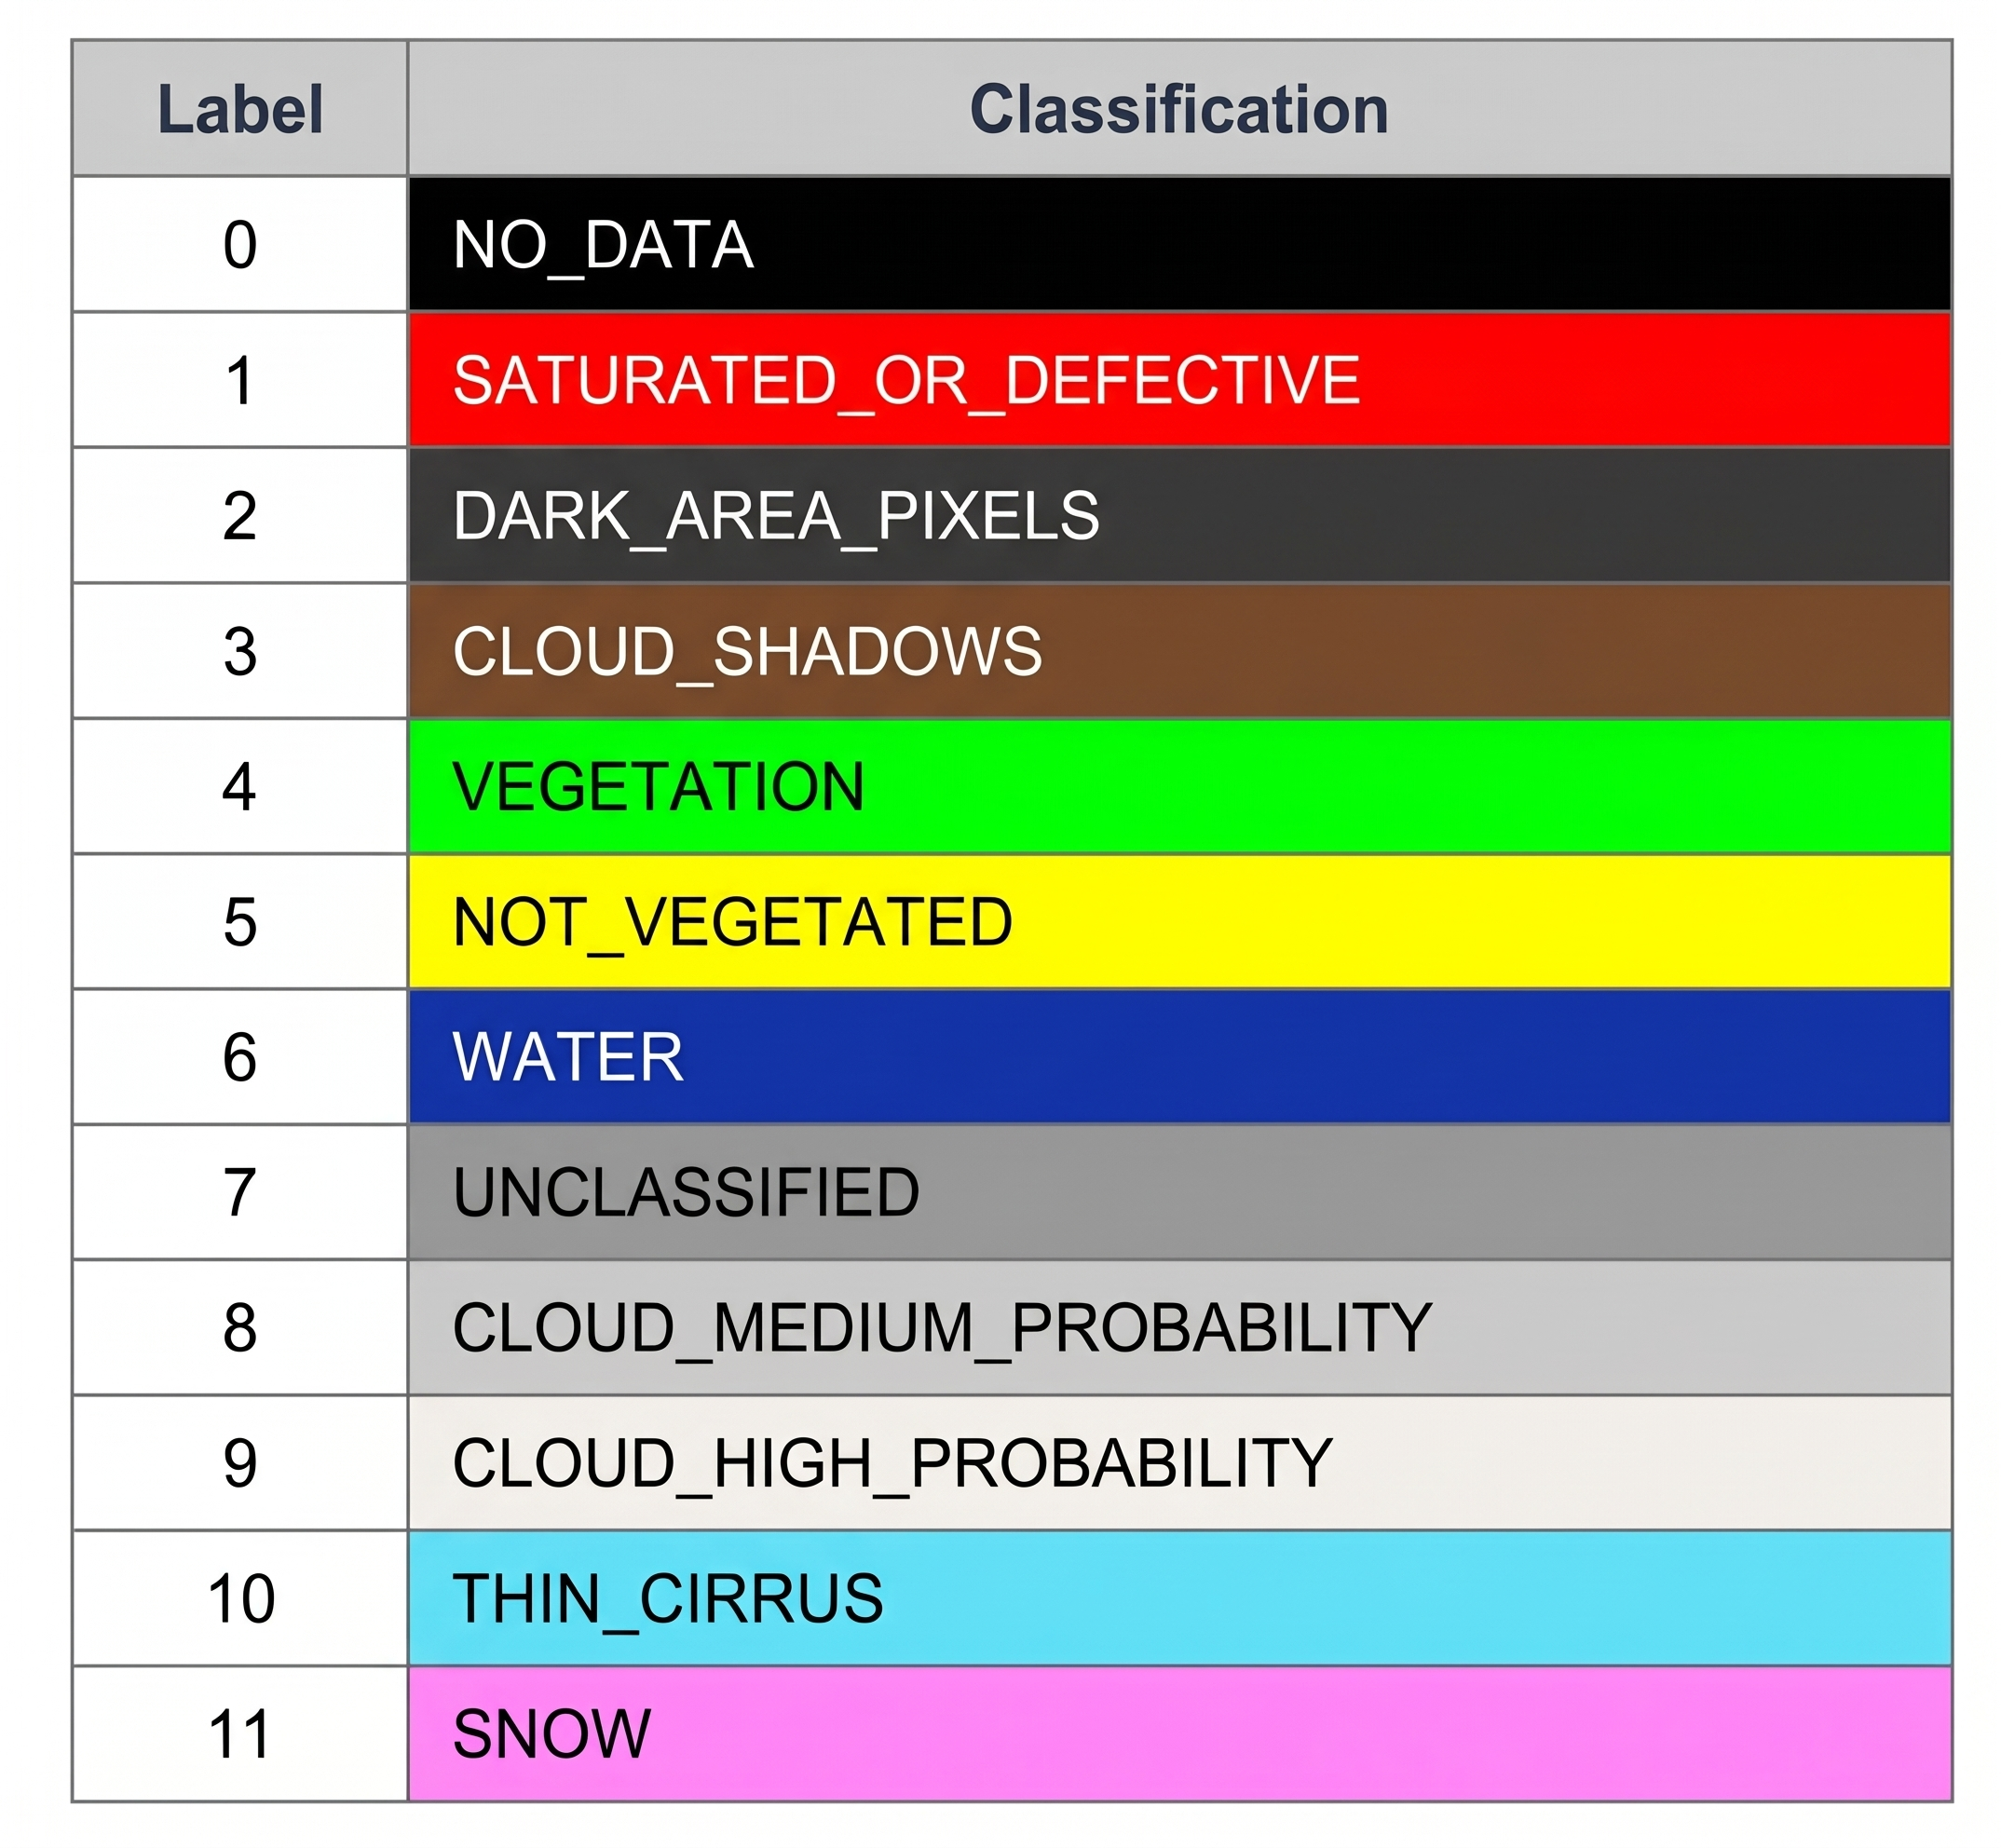
\includegraphics[width=0.4\textwidth]{figures/classes}
    \caption{Discrete classification labels and their corresponding land-cover categories.}
    \label{fig:labels}
\end{figure}

\begin{itemize}
    \item \textbf{Data Format:} Export the extracted data as a Tab-Separated Values (TSV) file.
    \item \textbf{Required Columns:} The final table must strictly include Latitude, Longitude, the 10 spectral band values, and the categorical class label derived from the polygon metadata.
\end{itemize}

\subsection{Model Implementation and Training}
Once the training dataset is prepared, students must implement and compare six distinct machine learning architectures. This comparative analysis evaluates how different mathematical approaches handle the high-dimensional spectral data of the selected scene. The performance of each model must be assessed using standard validation metrics, including the Confusion Matrix, Kappa Coefficient, Overall Accuracy, Precision, Recall, and F1-Score.

\begin{enumerate}
    \item \textbf{Logistic Regression (LR):} Serves as the linear baseline for performance comparison, predicting the probability of a categorical dependent variable.

    \item \textbf{K-Nearest Neighbors (KNN):} A non-parametric method that assigns class membership based on a plurality vote of its neighbors. Pixels are classified according to the most common category among the $k$ nearest training samples within the spectral feature space.

    \item \textbf{Naive Bayes (NB):} A probabilistic classifier based on Bayes' Theorem that assumes strong (naive) independence between the input spectral bands. It calculates the probability of each class given the observed pixel values and selects the most likely outcome.

    \item \textbf{Decision Trees (DT):} A logic-based model that utilizes a hierarchical tree structure to split data based on spectral thresholds. This approach is particularly useful for identifying which specific bands are most influential in distinguishing land-cover classes. It is highly recommended to extend this approach using ensemble methods, such as Random Forest or Gradient Boosting.

    \item \textbf{Support Vector Machines (SVM):} A kernel-based algorithm that identifies the optimal hyperplane to maximize the margin between class clusters in a multi-dimensional feature space. It is highly effective for complex classification tasks where classes are not linearly separable.

    \item \textbf{Artificial Neural Networks (ANN):} A computational model composed of interconnected layers of neurons designed to learn complex, non-linear relationships between spectral signatures and land-cover categories.
\end{enumerate}

\subsection{Model Comparison and Performance Evaluation}
To identify the most robust classification architecture, students must perform an exhaustive Hyperparameter Optimization (HPO) process. This involves systematically testing and adjusting the internal settings of each algorithm to maximize its predictive power for the specific study area.

Once the models are tuned, a rigorous performance assessment must be conducted by comparing their resulting Confusion Matrices. Students are required to compute and analyze the following evaluation metrics:
\begin{itemize}
    \item \textbf{Overall Accuracy:} To quantify the total percentage of correctly classified pixels.
    \item \textbf{Kappa Coefficient:} To measure the agreement between predicted and reference data beyond what is expected by chance.
    \item \textbf{Precision and Recall:} To assess the model's reliability and completeness for each land-cover category.
    \item \textbf{F1-Score:} To determine the harmonic balance between precision and recall, ensuring the model remains accurate across all classes.
\end{itemize}

Finally, all findings must be synthesized into a comprehensive summary table. This table should facilitate a direct comparison between the six implemented architectures, clearly highlighting the highest-performing model based on the statistical metrics listed above.

\subsection{Final Raster Prediction (Inference)}
The culmination of the classification pipeline is the generation of a comprehensive thematic land-cover map through full-scene inference. Once the optimal model has been identified and validated, having achieved the highest statistical performance across the assessed metrics, it must be deployed to classify the remaining pixels comprising the broader study area.

Unlike the training phase, which utilized a discrete Tab-Separated Values (TSV) dataset derived from targeted polygons, the inference phase requires the model to process the original multidimensional image stack. The algorithm evaluates each pixel, treating its ten spectral bands as input features to predict its most likely class membership. This operation effectively transforms raw, multispectral reflectance data into a new, single-band categorical image.

The output of this process must be exported as a georeferenced raster file (e.g., GeoTIFF or JP2 formats). In this final product, every pixel value corresponds to a specific integer code representing its predicted category (see Figure~\ref{fig:labels}). To ensure professional-grade results, the following requirements must be addressed:

\begin{itemize}
    \item \textbf{Spatial Consistency:} The final image must strictly retain the original Coordinate Reference System (CRS). This ensures perfectly aligned spatial predictions with the native satellite imagery and auxiliary geospatial layers.

    \item \textbf{Area Quantification:} Beyond visual representation, students are required to generate spatial statistics. Using the predicted categorical raster, calculate the total spatial area (in hectares or square kilometers) for each land-cover class.

    \item \textbf{Thematic Visualization:} Participants are encouraged to import the resulting GeoTIFF or JP2 into an open-source GIS environment, such as QGIS\footnote{\url{https://qgis.org/}} or other similar tool, to apply a discrete color symbology. This thematic visualization should clearly and intuitively distinguish between the different land-cover types.  See figure~\ref{fig:expected_output} as reference.
\end{itemize}

\begin{figure}
    \centering
    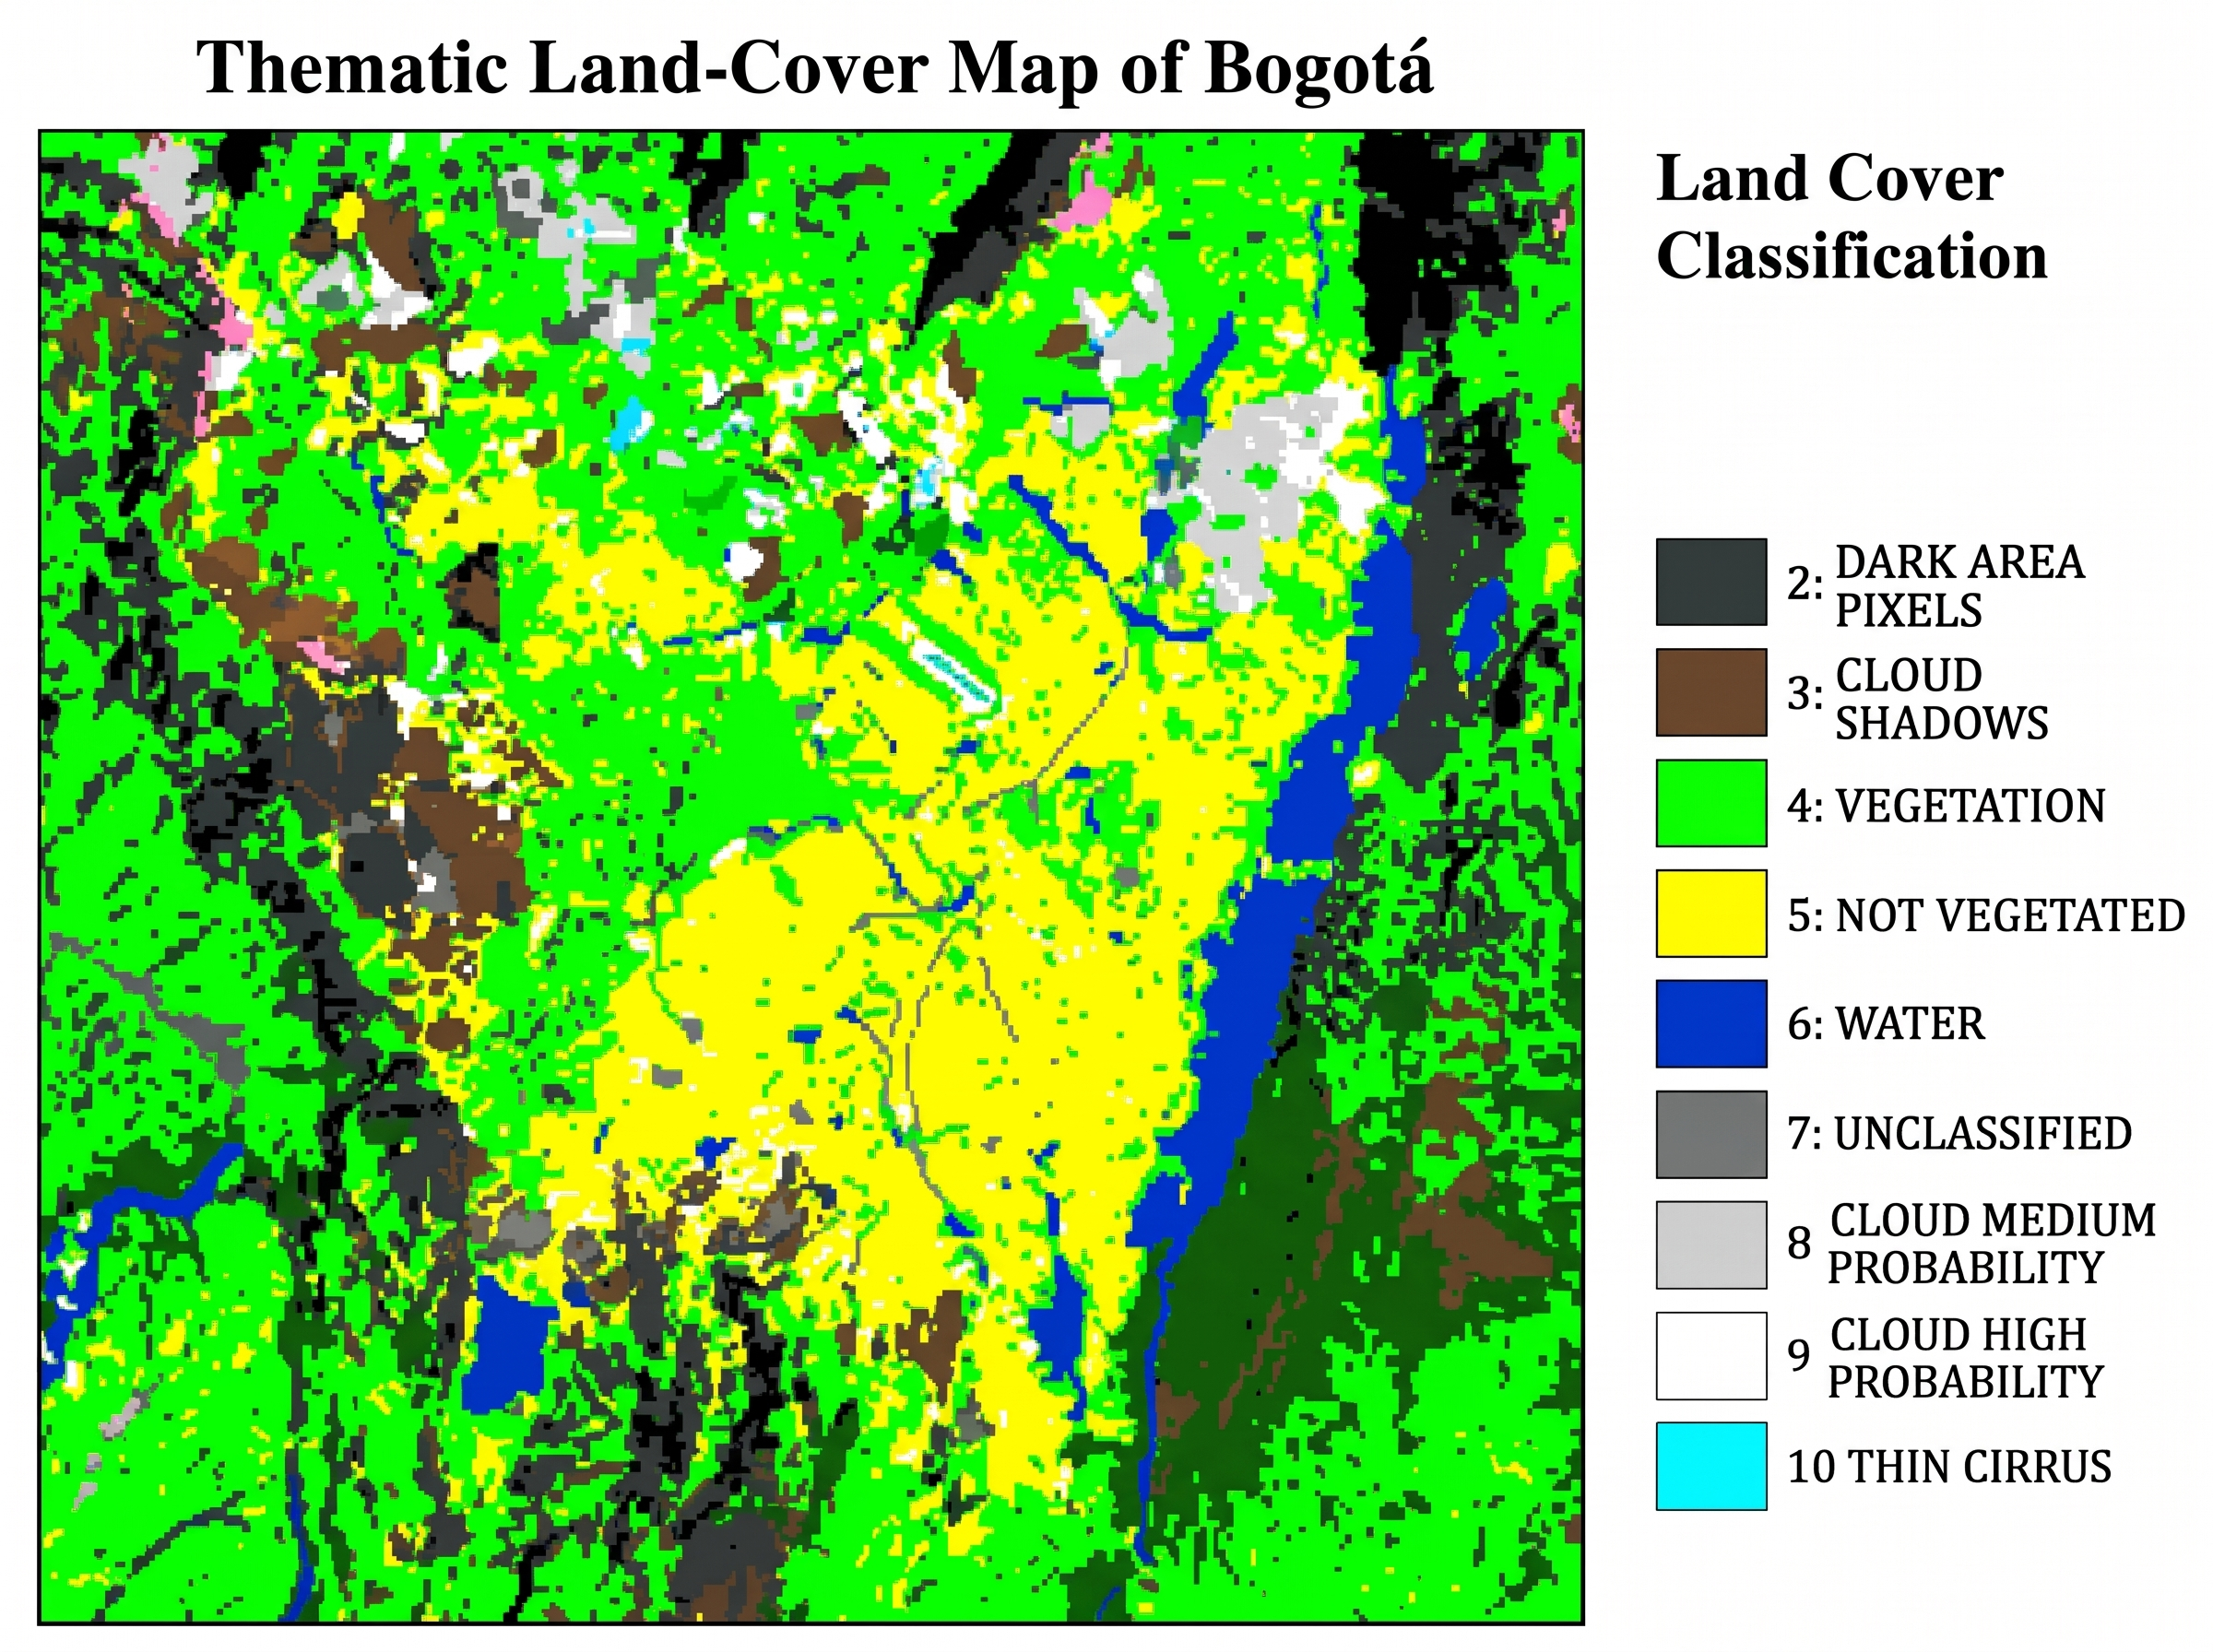
\includegraphics[width=0.75\textwidth]{figures/expected_output}
    \caption{Expected thematic land-cover map of Bogotá generated via full-scene spatial inference. The legend details the discrete land-cover classifications applied to the region of interest.}
    \label{fig:expected_output}
\end{figure}

\section{Project Phases and Weekly Deliverables}
The project is structured around two primary milestones, with specific components to be submitted at the conclusion of their respective weeks:

\subsection*{Phase 1: Pre-processing and Training (Week 2)}
This phase focuses on technical data preparation, feature extraction, and initial model testing.
\begin{itemize}
    \item \textbf{Deliverables:} A \textbf{PDF report} with the documentation of the TSV training dataset construction and preliminary evaluation metrics (specifically, the Confusion Matrix and Overall Accuracy) for a minimum of \textbf{three} implemented classification architectures.
    \item \textbf{Deadline:} November 13, 2026. Midnight.
\end{itemize}

\subsection*{Phase 2: Synthesis and Prediction (Week 4)}
This final phase encompasses model optimization, full-scene spatial inference, and comprehensive reporting.
\begin{itemize}
    \item \textbf{Deliverables:} The predicted thematic raster exported as a georeferenced image (GeoTIFF or JP2), the complete technical report detailing the comparative analysis (PDF and \LaTeX), and a compressed archive (ZIP or TAR.GZ) containing all reproducible source code.
    \item \textbf{Deadline:} November 27, 2026. 7:00PM.
\end{itemize}

\section{Conclusion}
This project represents a complete synthesis of the applied GeoAI pipeline, guiding students from raw multispectral data acquisition to advanced spatial inference. By leveraging computational environments to extract Sentinel-2 spectral signatures, optimize machine learning architectures, and generate thematic land-cover maps, participants successfully bridge the gap between theoretical data science and practical geoinformatics. Beyond the technical execution of data extraction and algorithmic tuning, the ultimate value of this exercise lies in producing rigorous, actionable environmental intelligence. As students finalize their spatial statistics and thematic visualizations, they transition from passive observers of geospatial data into capable architects of modern environmental monitoring systems.

\end{document}
